\chapter{Sprint 3: Breakdown Management and Intervention Planning}

\section{Introduction}

The third sprint focuses on developing the breakdown management and intervention planning modules, which are critical components for maintaining telecommunications network infrastructure. This sprint addresses both reactive and proactive aspects of network maintenance by implementing systems for reporting and tracking network failures while enabling preventive maintenance through scheduled interventions.

Network breakdowns represent urgent situations requiring immediate attention, such as power outages, equipment failures, or connectivity losses that can significantly impact service quality and affect thousands of users. The intervention planning module enables managers and engineers to schedule preventive maintenance tasks, assign technicians, and track activities. Together, these modules create a comprehensive maintenance management system balancing reactive problem-solving with proactive prevention strategies.

\section{Sprint Backlog}

Table \ref{tab:sprint3-backlog} presents the Sprint 3 backlog with eight main user stories covering breakdown management and intervention planning functionalities.

\begin{table}[H]
\centering
\scriptsize
\caption{Sprint 3 Backlog - Breakdown and Intervention Management}
\label{tab:sprint3-backlog}
\begin{tabular}{|p{2.8cm}|p{4cm}|p{5cm}|c|c|}
\hline
\textbf{Functionality} & \textbf{User Story} & \textbf{Tasks} & \textbf{Complexity} & \textbf{Hours} \\
\hline
Report Breakdown & As an engineer, I want to report network breakdowns for quick resolution & Create breakdown form, implement severity classification, auto-capture downtime start & High & 8h \\
\hline
Assign Breakdown & As a manager, I want to assign breakdowns to technicians & Implement assignment logic, send notifications, update status & Medium & 5h \\
\hline
Track Resolution & As a technician, I want to update breakdown status & Create status update interface, implement workflow transitions & Medium & 6h \\
\hline
Monitor Impact & As a manager, I want to see breakdown impact metrics & Display impacted users, calculate downtime, show statistics & Medium & 5h \\
\hline
Schedule Intervention & As an engineer, I want to schedule maintenance interventions & Create intervention form, check availability, prevent conflicts & High & 7h \\
\hline
Assign Technician & As a manager, I want to assign technicians to interventions & Implement assignment interface, check workload, send notifications & Medium & 5h \\
\hline
Update Status & As a technician, I want to update intervention progress & Create status interface, implement workflow, capture completion & Low & 4h \\
\hline
View History & As a manager, I want to view maintenance history & Create history view, filter by criteria, display statistics & Medium & 6h \\
\hline
\multicolumn{4}{|r|}{\textbf{Total:}} & \textbf{46h} \\
\hline
\end{tabular}
\end{table}

\section{Class Diagram}

Figure \ref{fig:sprint3-class} illustrates the class diagram introducing two core entities: \texttt{Breakdown} and \texttt{Intervention}, which work with existing entities for comprehensive maintenance management.

\begin{figure}[H]
\centering
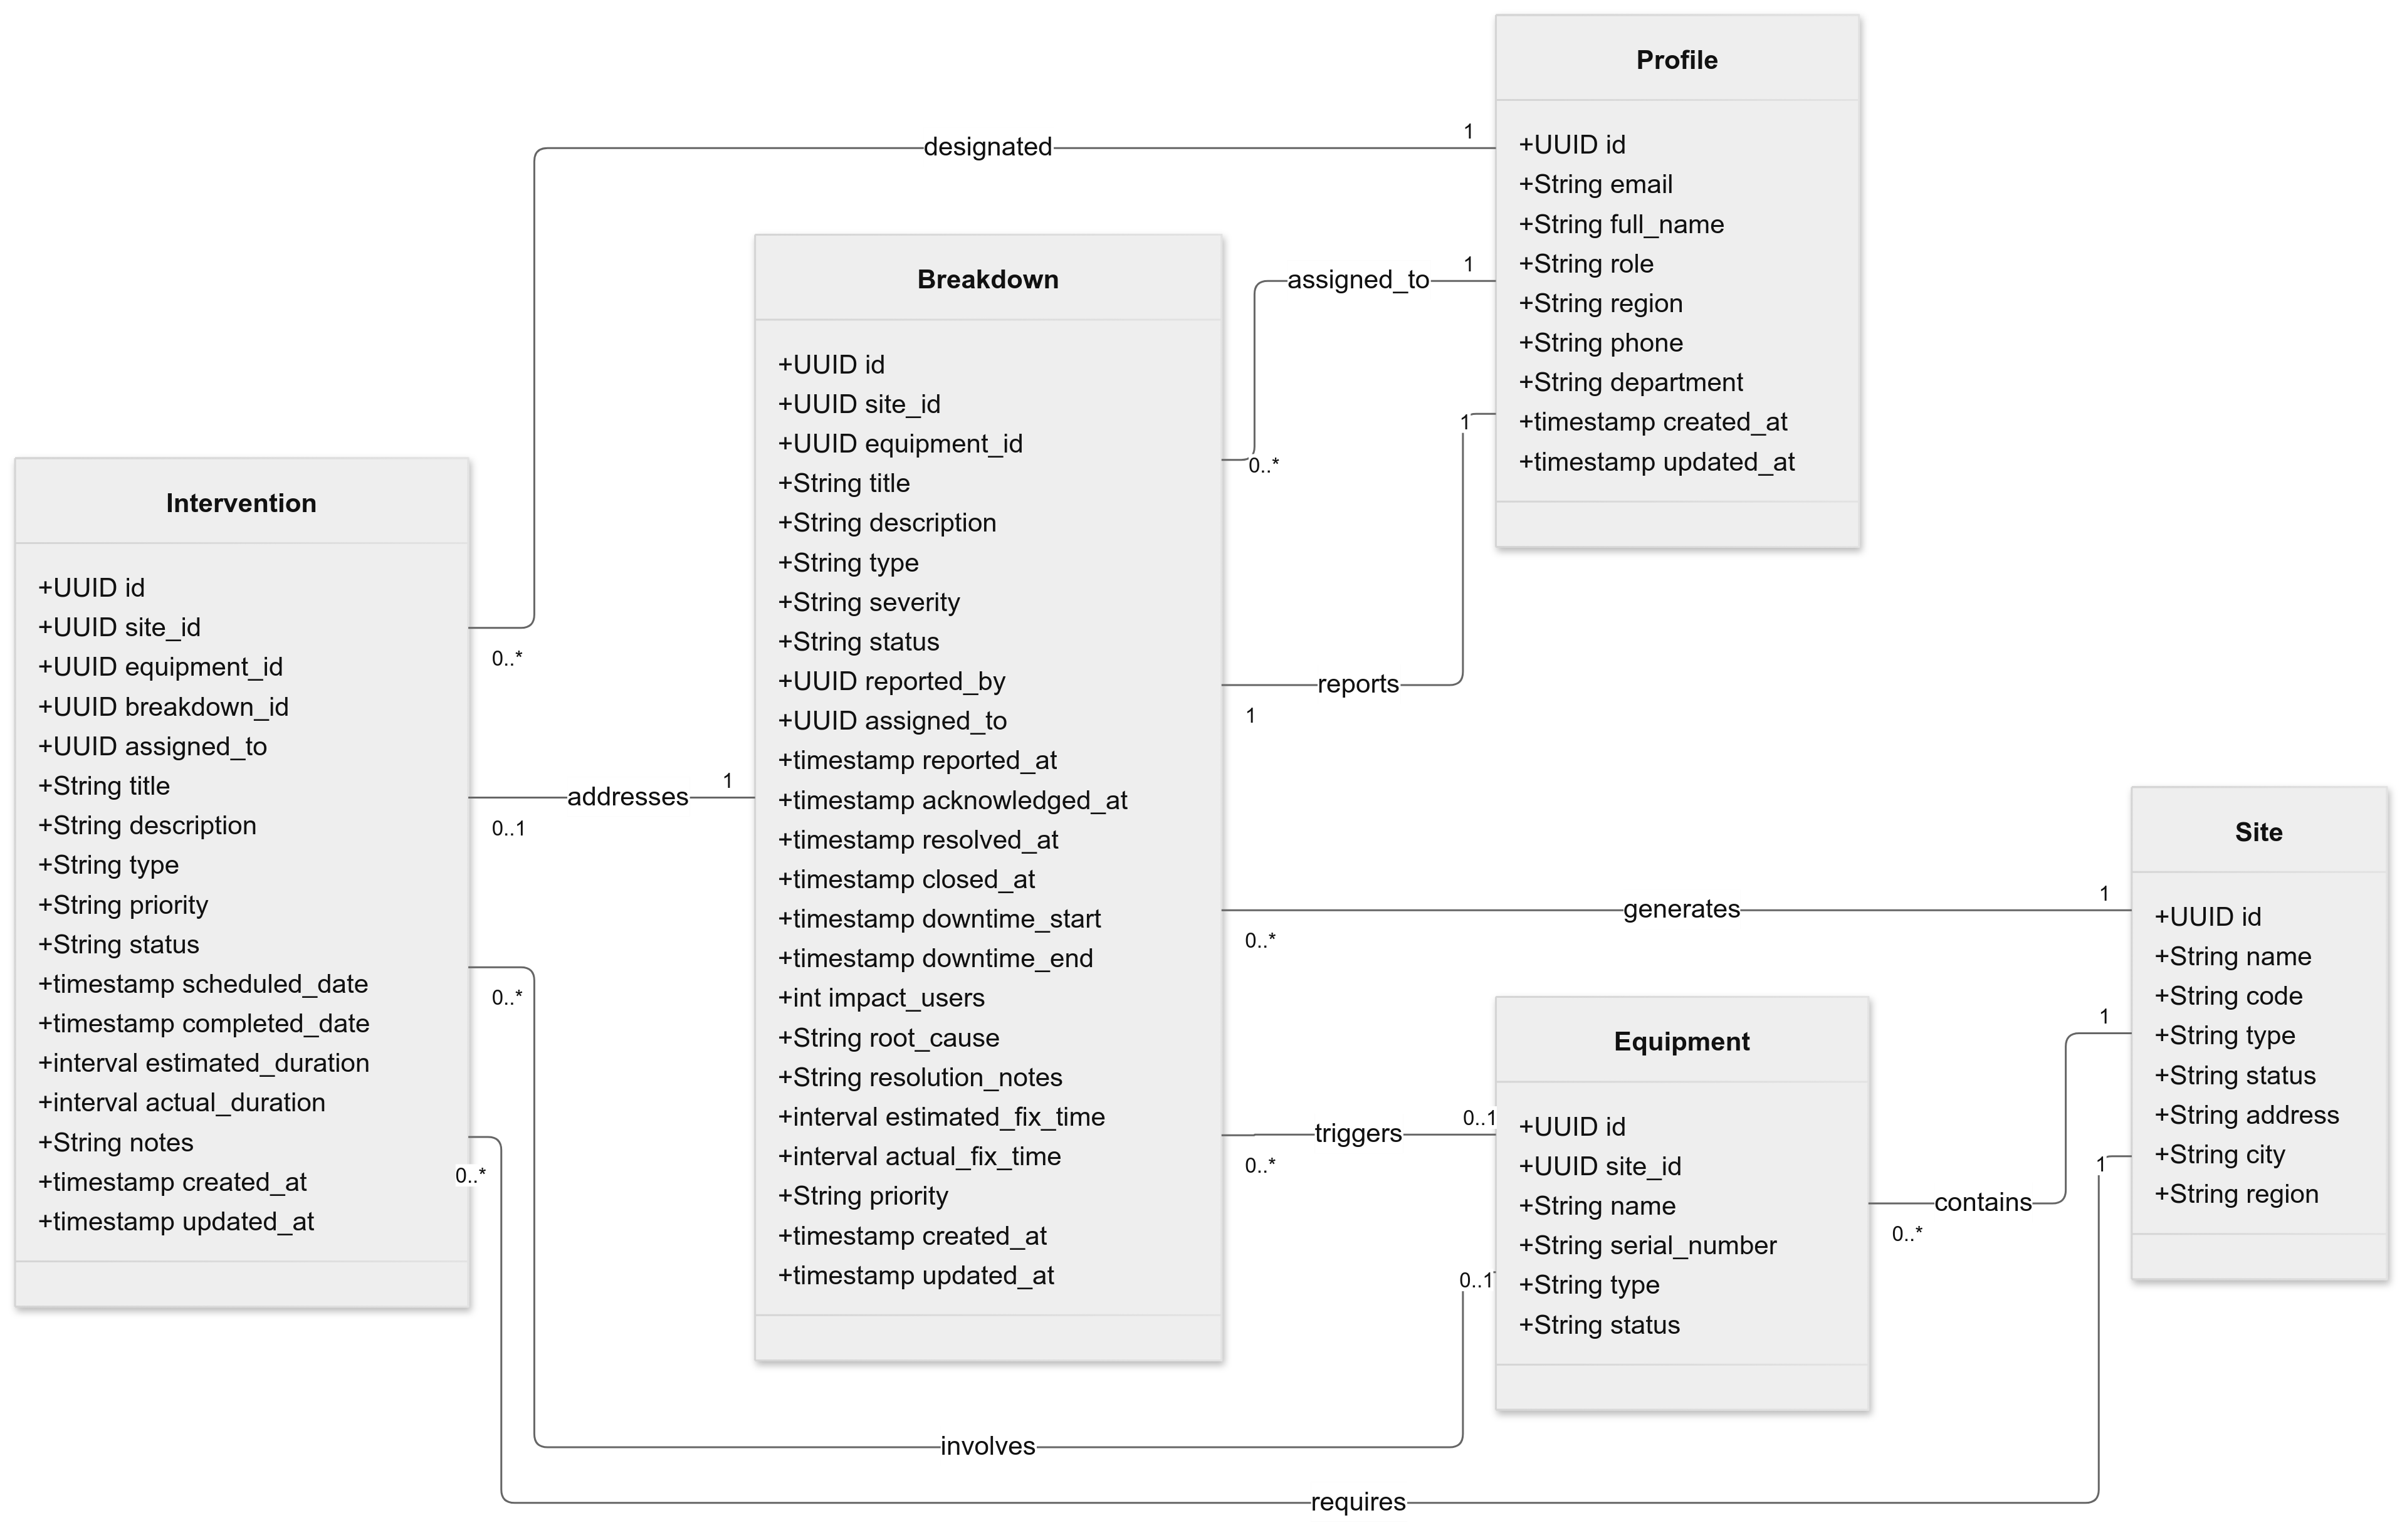
\includegraphics[width=0.7\textwidth]{img/chap_05/sprint3_class_diagram.png}
\caption{Class diagram for breakdown and intervention management}
\label{fig:sprint3-class}
\end{figure}

The \texttt{Breakdown} class represents network failures requiring immediate attention, tracking problem type, severity level (minor, major, critical), and status (open, investigating, in progress, resolved, closed). It maintains timestamps for the entire lifecycle and tracks user impact through \texttt{impact\_users} and downtime duration. The \texttt{Intervention} class manages scheduled maintenance activities, categorizing by type (preventive, corrective, installation, replacement) and priority. Both classes maintain relationships with \texttt{Profile}, \texttt{Site}, and \texttt{Equipment} entities, ensuring proper association with network infrastructure.

\section{Use Case Diagram}

Figure \ref{fig:sprint3-usecase} presents the use case diagram employing inheritance-based permission hierarchy where each role inherits all capabilities from roles below while adding specific functionalities.

\begin{figure}[H]
\centering
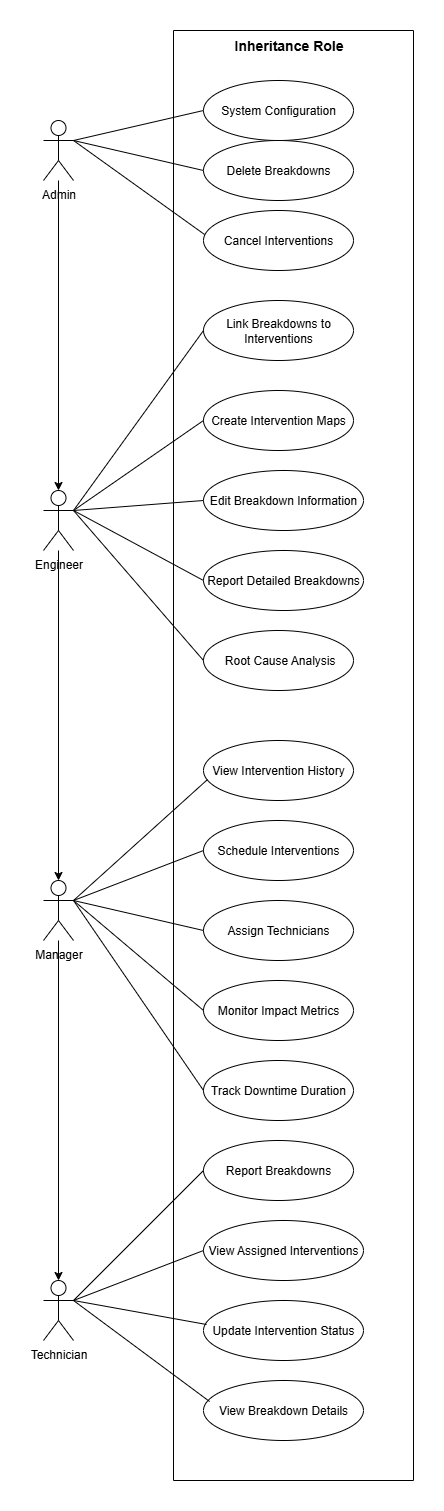
\includegraphics[width=0.7\textwidth]{img/chap_05/sprint3_usecase_diagram.png}
\caption{Use case diagram with role inheritance for Sprint 3}
\label{fig:sprint3-usecase}
\end{figure}

\textbf{Field Technicians} have base operational capabilities: view assigned interventions, update intervention status, report breakdowns, and view breakdown details. \textbf{Managers} inherit technician capabilities and add supervisory functions including viewing statistics, scheduling interventions, and assigning technicians. \textbf{Network Engineers} inherit manager capabilities and add technical analysis including root cause analysis and detailed planning. \textbf{Administrators} possess all privileges plus system management capabilities including deletion and configuration rights.

\section{Use Case Permissions Table}

Table \ref{tab:sprint3-permissions} details the permission matrix using Yes/No values indicating each role's capabilities within the inheritance hierarchy.

\begin{table}[H]
\centering
\scriptsize
\caption{Sprint 3 Use Case Permissions by Role}
\label{tab:sprint3-permissions}
\begin{tabular}{|p{5.5cm}|c|c|c|c|}
\hline
\textbf{Use Case} & \textbf{Technician} & \textbf{Manager} & \textbf{Engineer} & \textbf{Admin} \\
\hline
View Assigned Interventions & Yes & Yes & Yes & Yes \\
\hline
Update Intervention Status & Yes & Yes & Yes & Yes \\
\hline
Report Breakdowns & Yes & Yes & Yes & Yes \\
\hline
View Breakdown Details & Yes & Yes & Yes & Yes \\
\hline
View Intervention Statistics & No & Yes & Yes & Yes \\
\hline
View Breakdown Reports & No & Yes & Yes & Yes \\
\hline
Schedule Interventions & No & Yes & Yes & Yes \\
\hline
Assign Technicians & No & Yes & Yes & Yes \\
\hline
Track Downtime Duration & No & Yes & Yes & Yes \\
\hline
Monitor Impact Metrics & No & Yes & Yes & Yes \\
\hline
Root Cause Analysis & No & No & Yes & Yes \\
\hline
Create Intervention Plans & No & No & Yes & Yes \\
\hline
Edit Breakdown Information & No & No & Yes & Yes \\
\hline
Link Breakdowns to Equipment & No & No & Yes & Yes \\
\hline
Delete Breakdowns & No & No & No & Yes \\
\hline
Delete Interventions & No & No & No & Yes \\
\hline
Cancel Interventions & No & No & No & Yes \\
\hline
System Configuration & No & No & No & Yes \\
\hline
\end{tabular}
\end{table}

\section{Use Case Description}

Table \ref{tab:sprint3-usecase-detail} provides detailed description of the "Report Breakdown" use case.

\begin{table}[H]
\centering
\scriptsize
\caption{Detailed Description - Report Breakdown Use Case}
\label{tab:sprint3-usecase-detail}
\begin{tabular}{|p{3cm}|p{10.5cm}|}
\hline
\textbf{Element} & \textbf{Description} \\
\hline
\textbf{Use Case Name} & Report Breakdown \\
\hline
\textbf{Actor} & Network Engineer, Manager, Field Technician \\
\hline
\textbf{Description} & Allows users to report network breakdowns and failures requiring immediate attention with all necessary details for quick resolution \\
\hline
\textbf{Preconditions} & User authenticated with engineer/manager/technician role; Active sites exist; Breakdown types configured \\
\hline
\textbf{Postconditions} & Breakdown record created; Downtime tracking started; Notifications sent; Critical alerts escalated \\
\hline
\textbf{Main Flow} & 1. User clicks "Report Breakdown" button \newline 2. System displays breakdown form \newline 3. User enters title, description, type, and severity \newline 4. User selects affected site and equipment \newline 5. User estimates impacted users and fix time \newline 6. User submits form \newline 7. System validates required fields \newline 8. System creates breakdown with auto-captured timestamp \newline 9. System shows success confirmation \\
\hline
\textbf{Alternative Flow} & \textbf{A1 - Critical Severity:} At step 6, if severity is "Critical", system immediately notifies managers and highlights breakdown with urgent flag \newline \textbf{A2 - Equipment Selection:} At step 4, system loads equipment for selected site \\
\hline
\textbf{Exception Flow} & \textbf{E1 - Missing Fields:} At validation, if required fields empty, show error and return to form \newline \textbf{E2 - Invalid Data:} If negative values entered, show validation error \\
\hline
\end{tabular}
\end{table}

\section{Sequence Diagrams}

\subsection{Schedule Intervention Sequence}

Figure \ref{fig:sprint3-seq1} shows the interaction flow when scheduling a new maintenance intervention with conflict detection.

\begin{figure}[H]
\centering
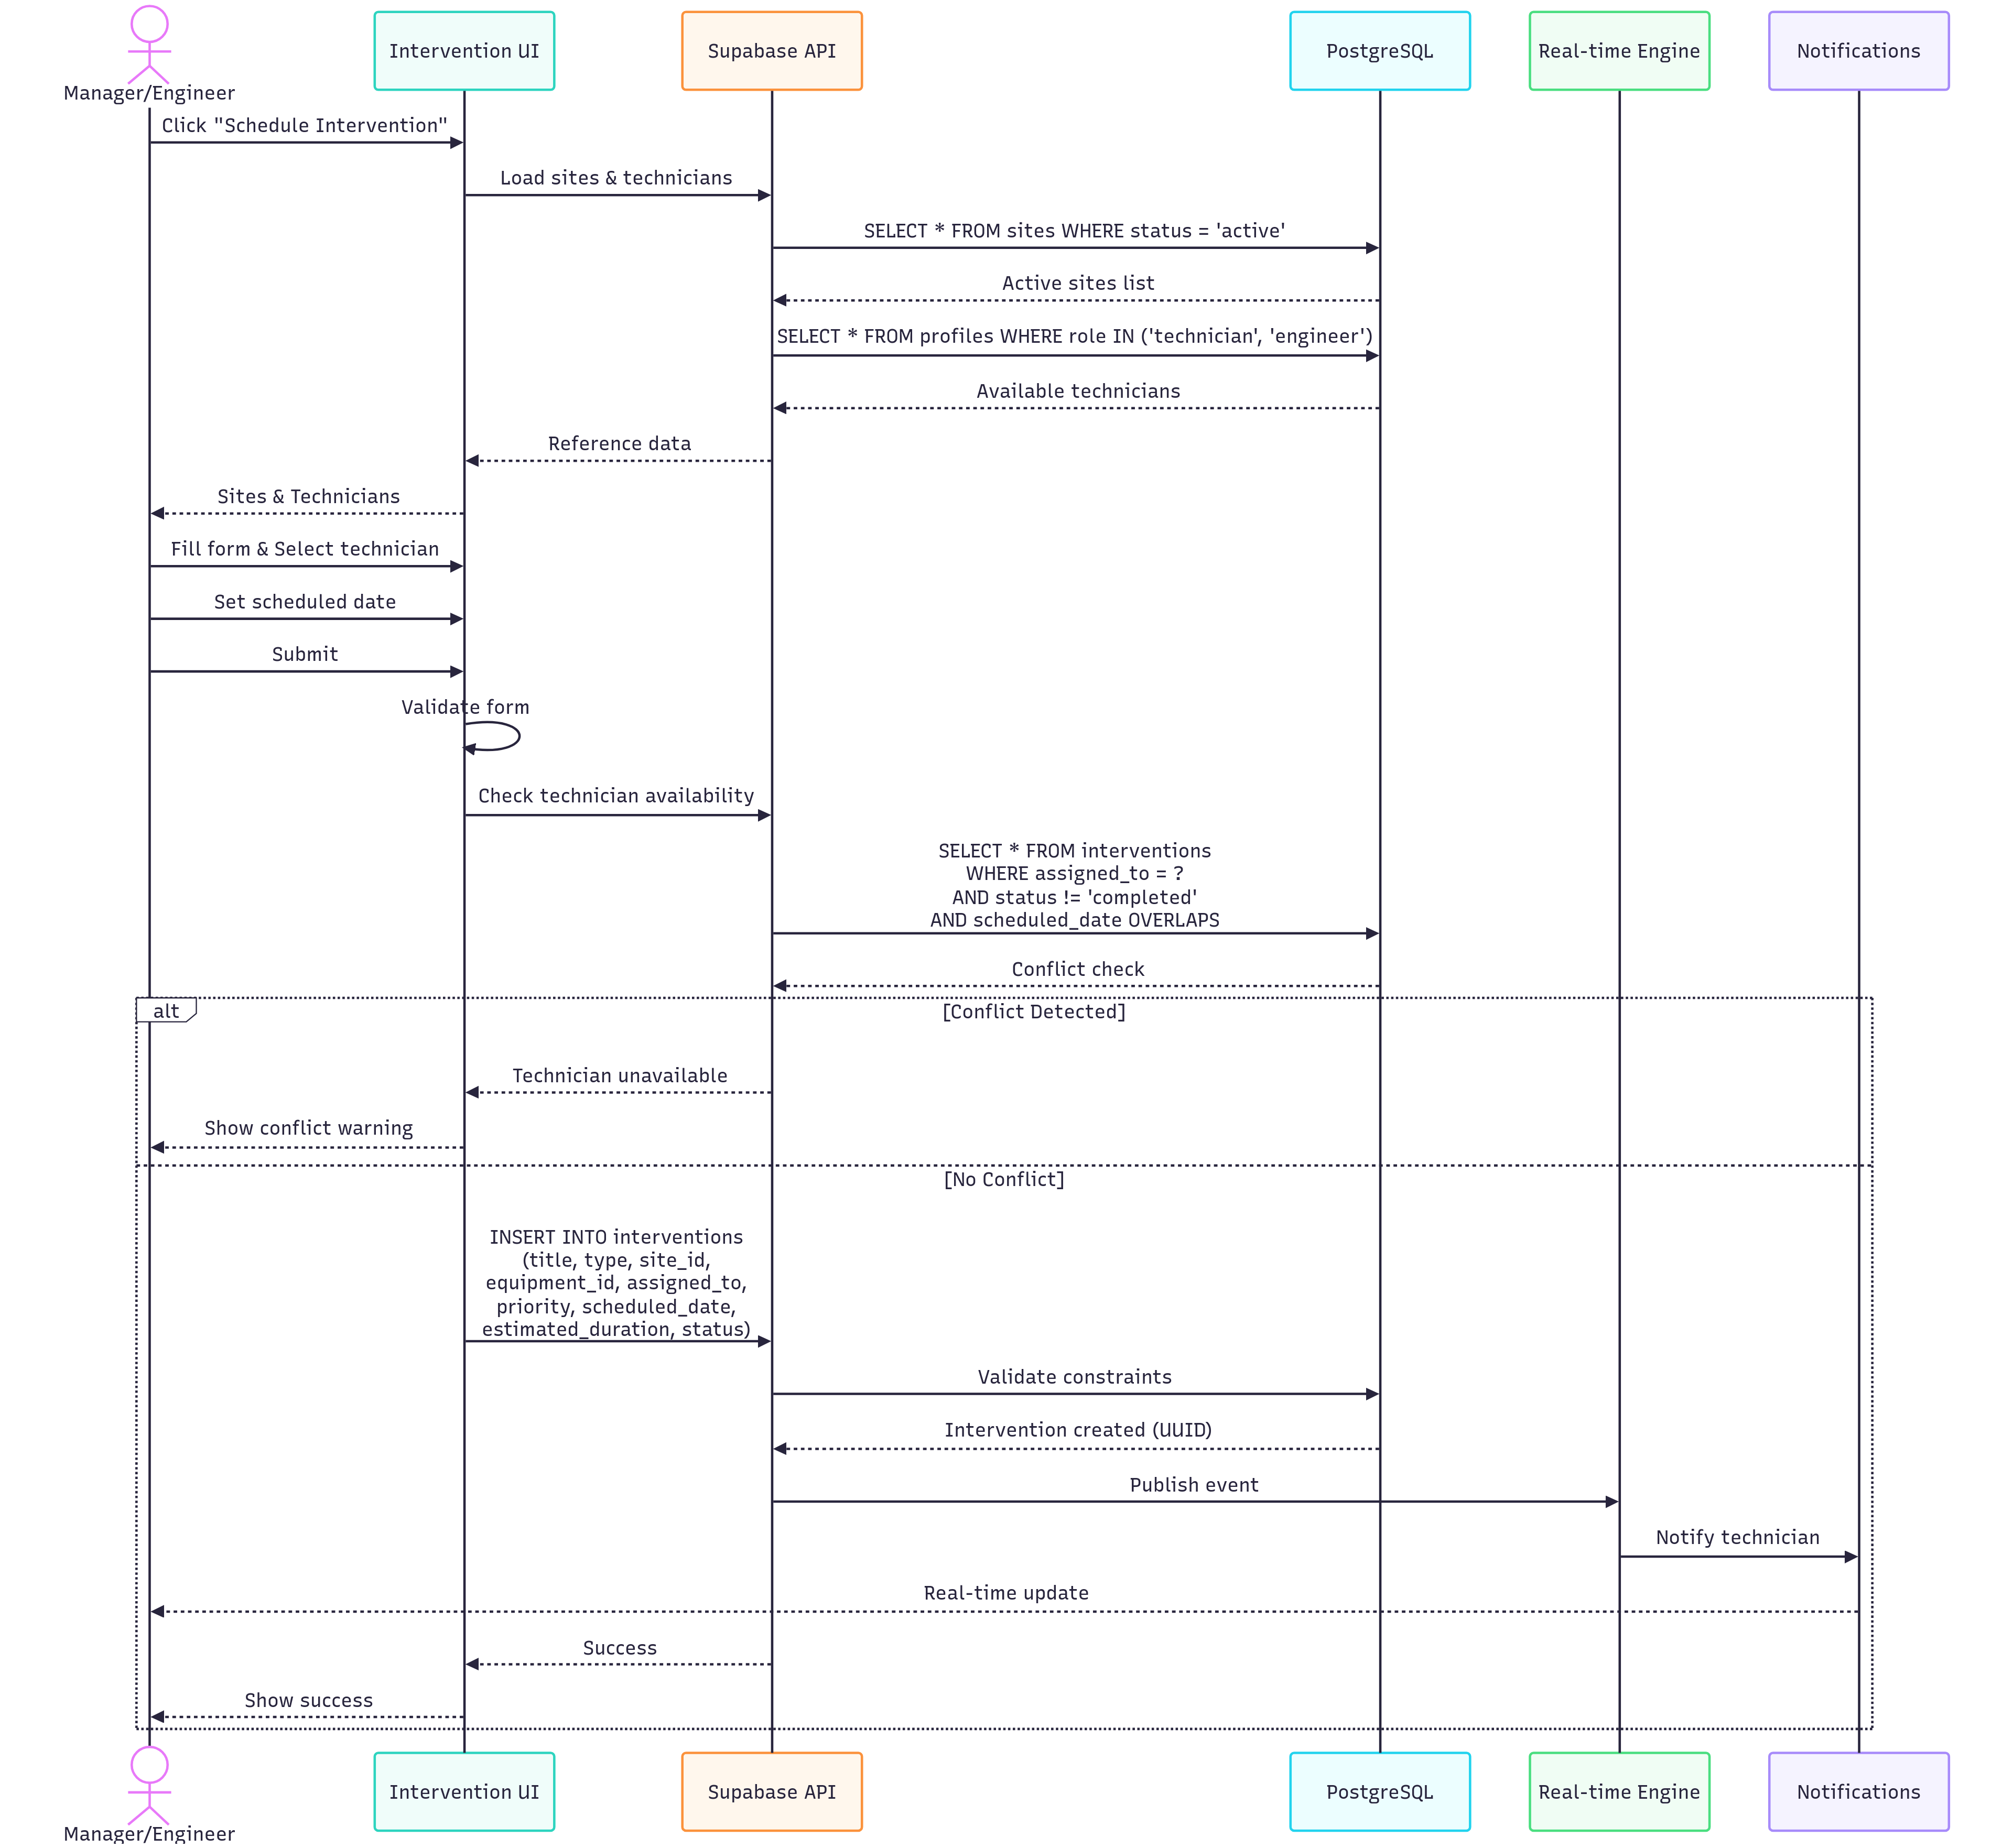
\includegraphics[width=0.7\textwidth]{img/chap_05/sprint3_sequence_intervention.png}
\caption{Sequence diagram for scheduling an intervention}
\label{fig:sprint3-seq1}
\end{figure}

\subsection{Report Breakdown Sequence}

Figure \ref{fig:sprint3-seq2} illustrates the workflow for reporting a network breakdown including critical severity escalation.

\begin{figure}[H]
\centering
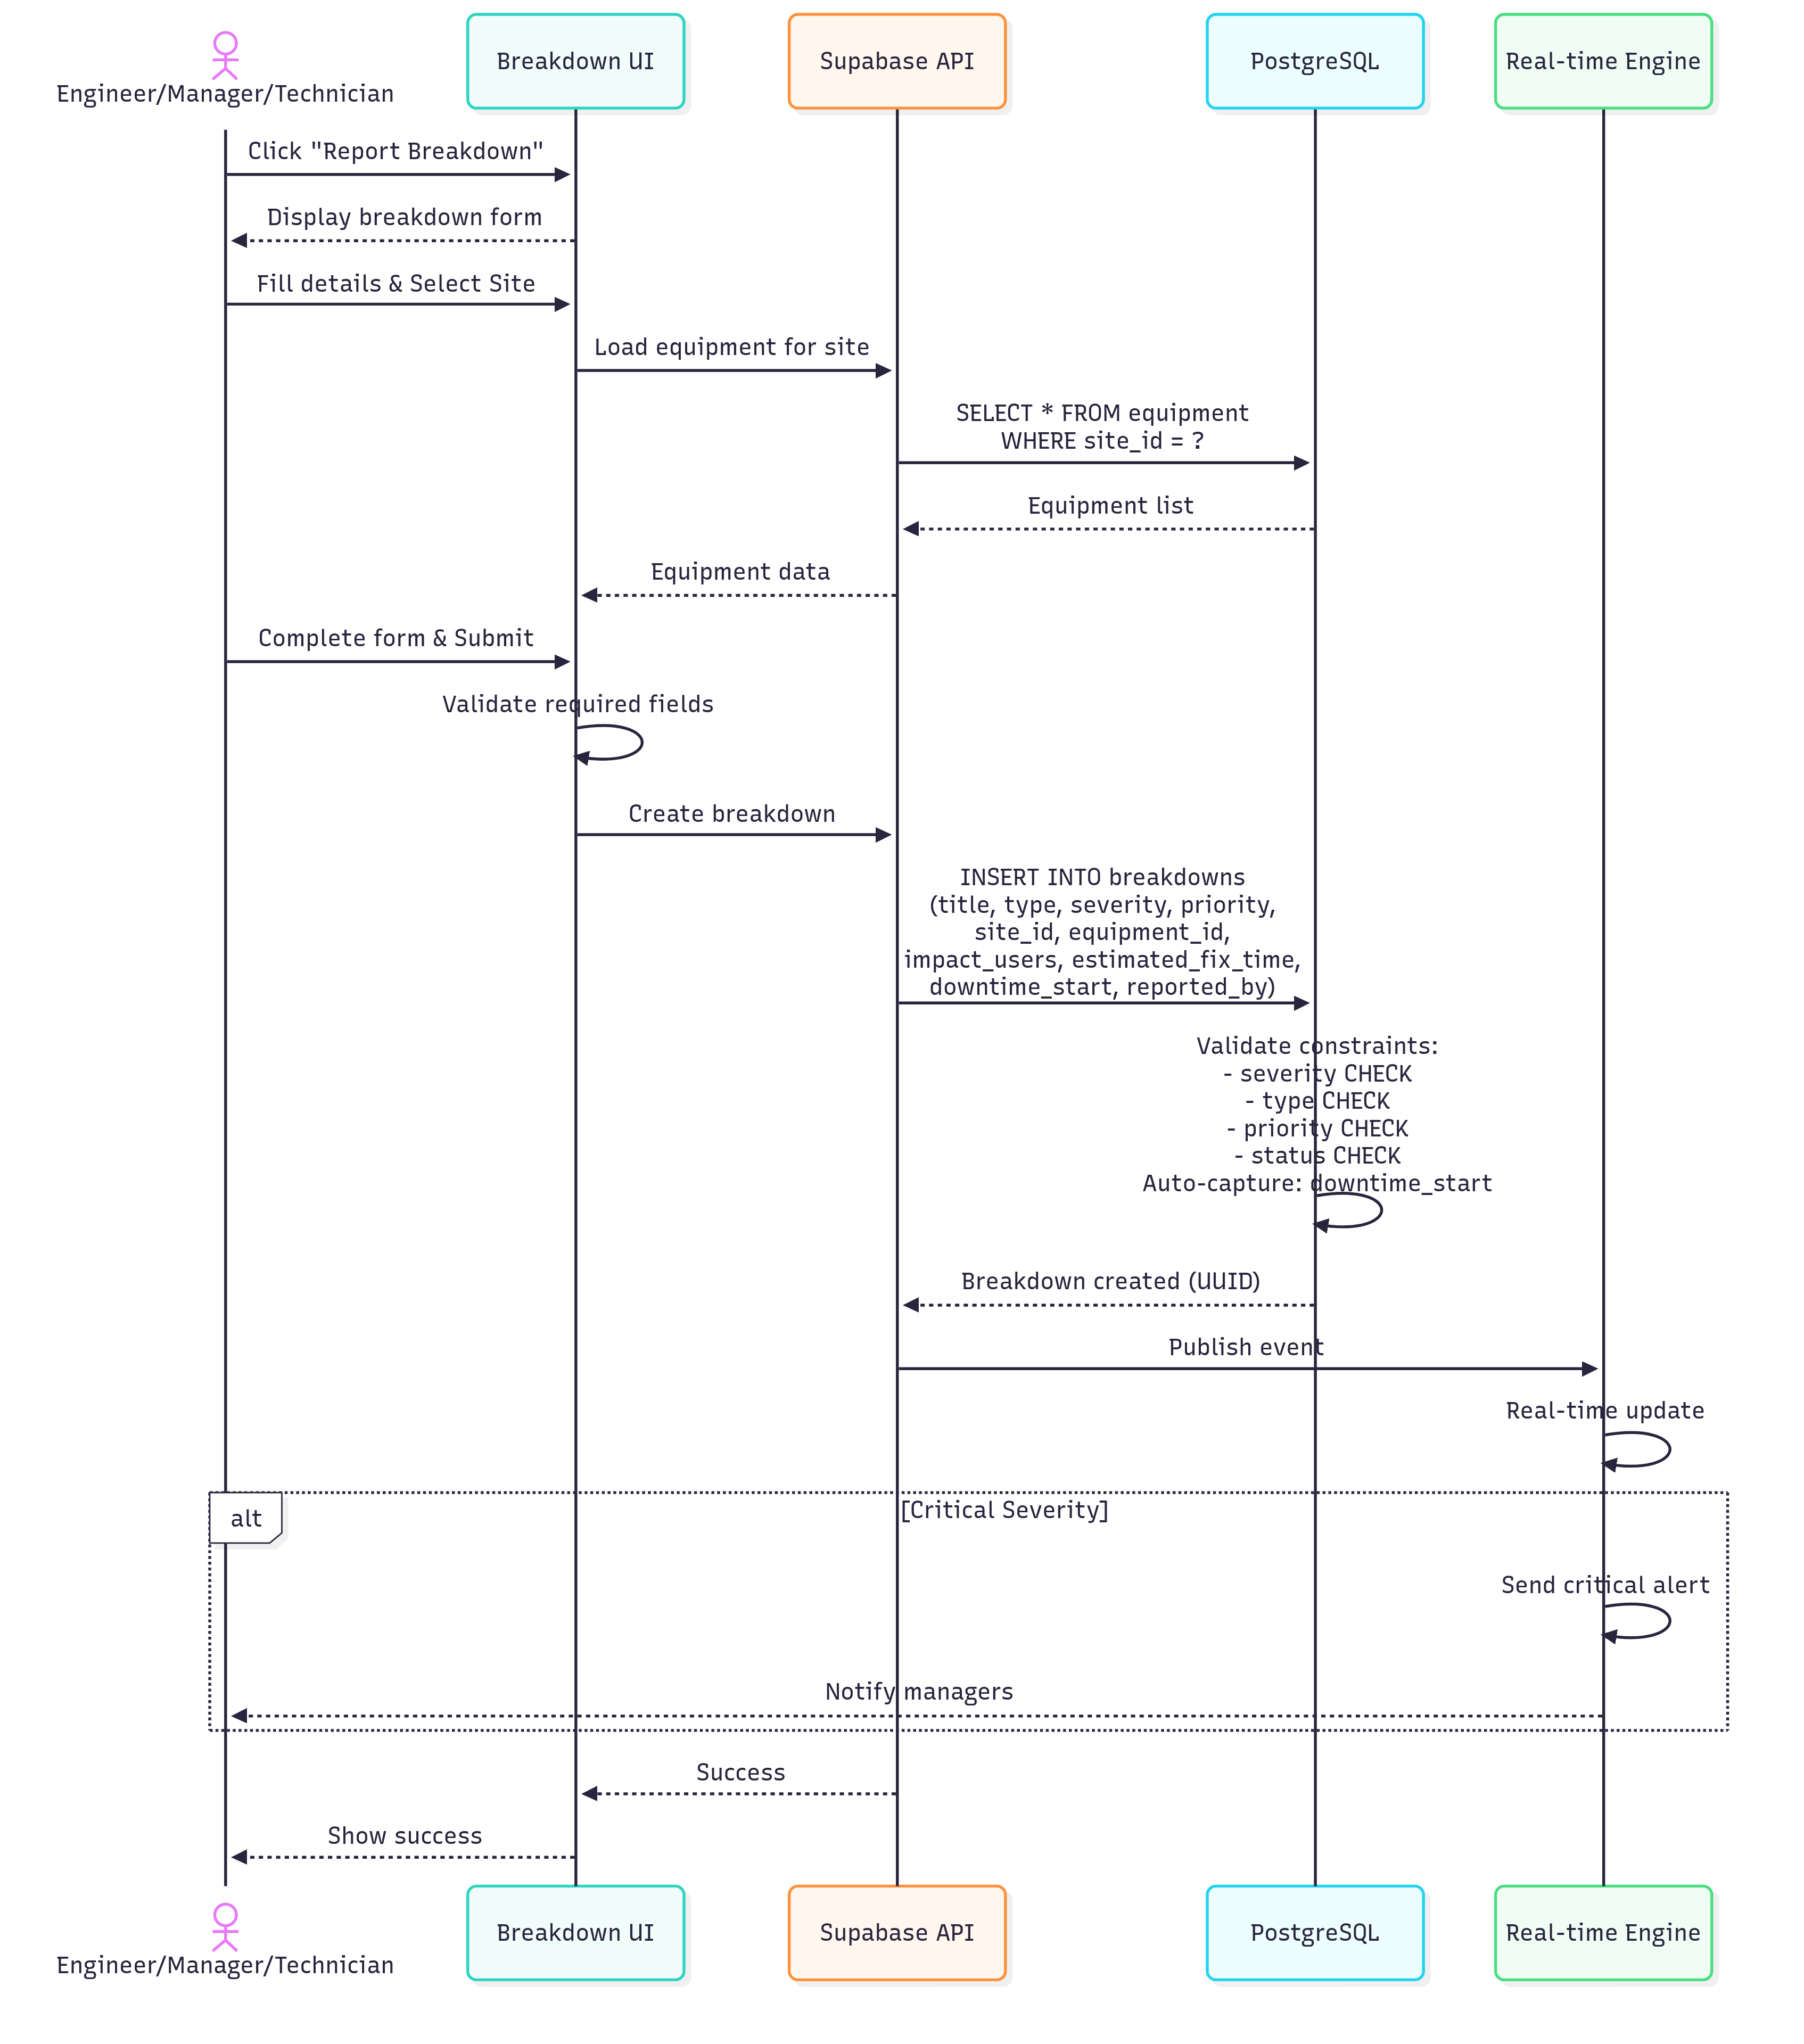
\includegraphics[width=0.7\textwidth]{img/chap_05/sprint3_sequence_breakdown.png}
\caption{Sequence diagram for reporting a breakdown}
\label{fig:sprint3-seq2}
\end{figure}

\section{Implementation}

This section presents the implemented interfaces for breakdown management and intervention planning modules.

\subsection{Intervention Management Dashboard}

Figure \ref{fig:sprint3-impl1} shows the intervention management interface with quick statistics and task listing.

\begin{figure}[H]
\centering
\fbox{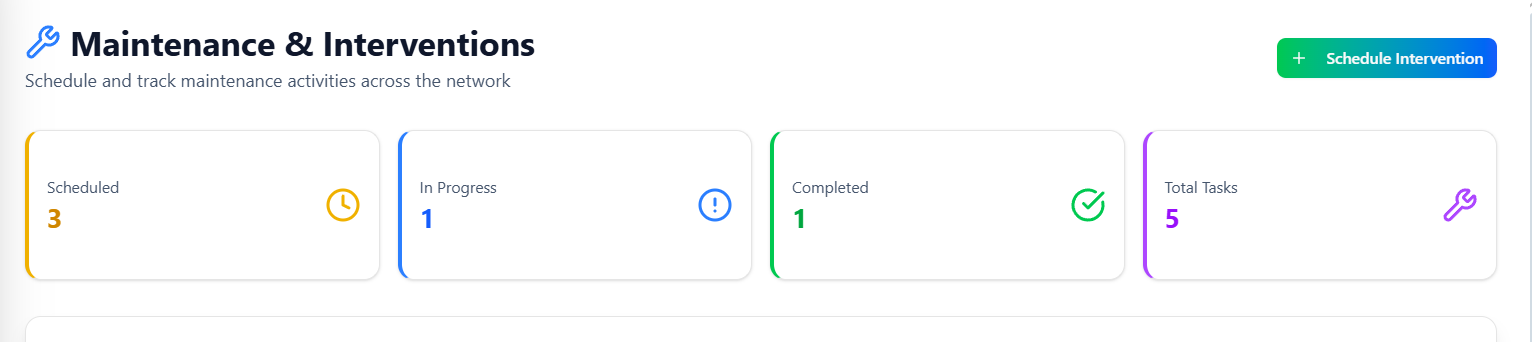
\includegraphics[width=0.70\textwidth]{img/chap_05/screenshot_interventions_dashboard.png}}
\caption{Intervention management dashboard with statistics and task list}
\label{fig:sprint3-impl1}
\end{figure}

The dashboard displays quick statistics showing scheduled, in-progress, and completed interventions. The interventions table presents each task with type, priority, status, site, assigned technician, and scheduled date using color-coded badges for quick identification.

\subsection{Breakdown Management Dashboard}

Figure \ref{fig:sprint3-impl2} displays the breakdown management interface tracking network failures.

\begin{figure}[H]
\centering
\fbox{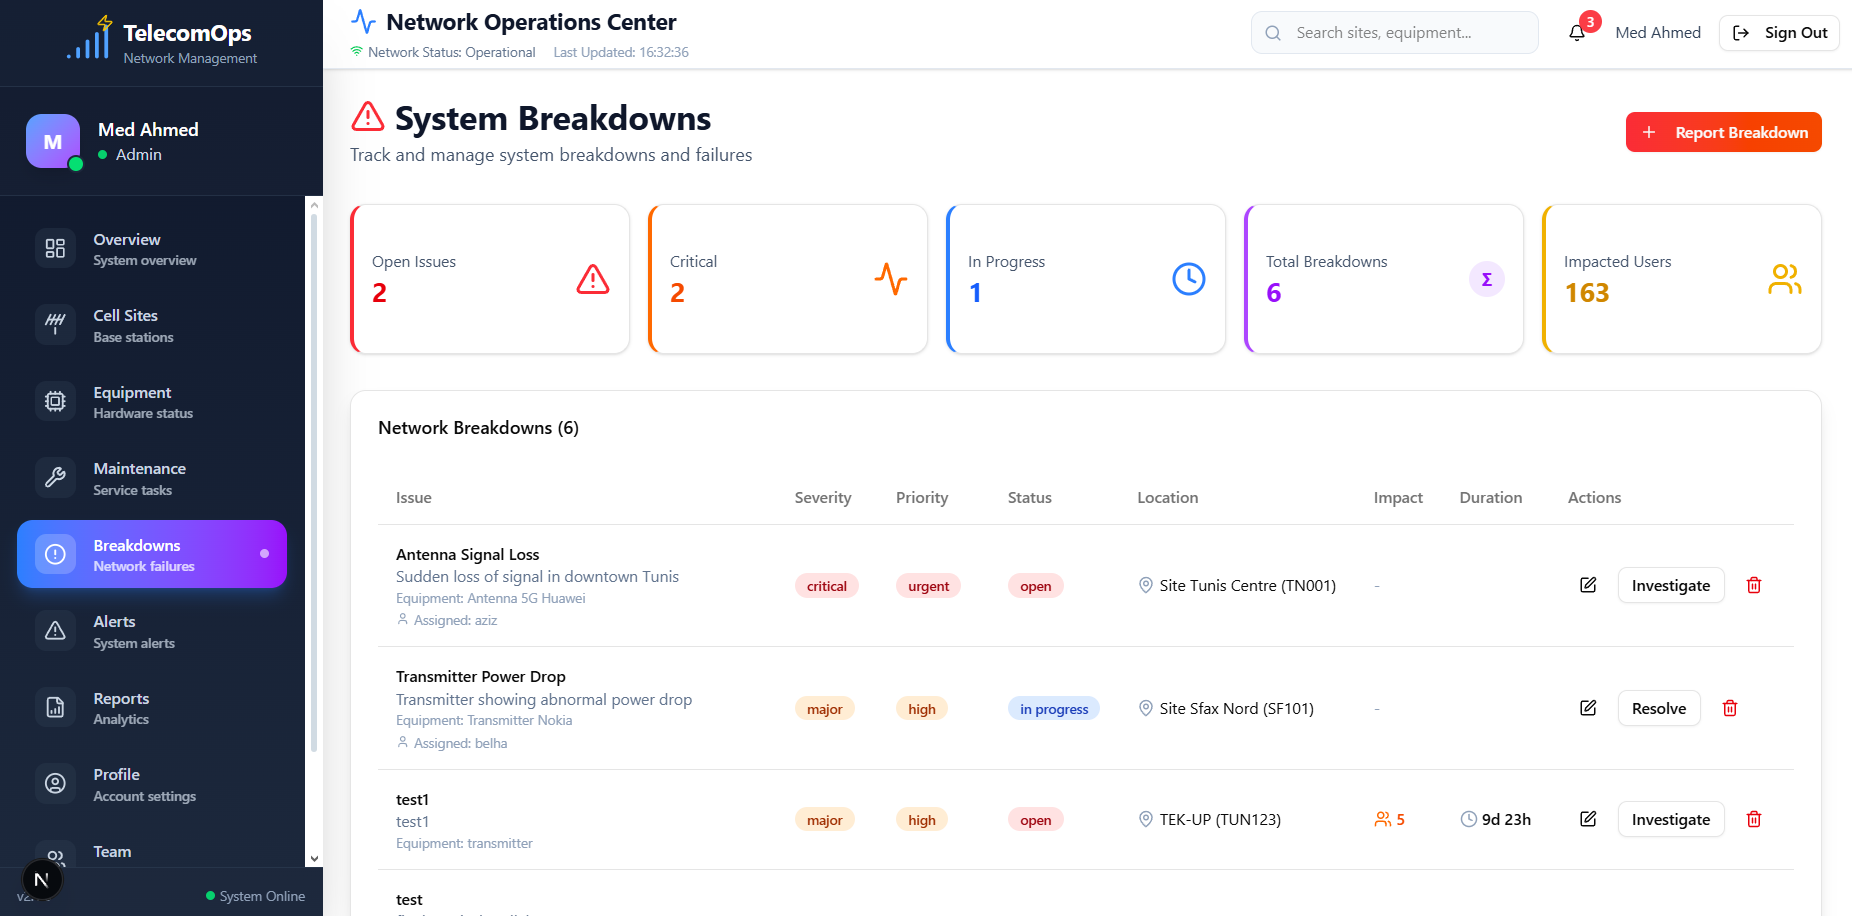
\includegraphics[width=0.70\textwidth]{img/chap_05/screenshot_breakdowns_dashboard.png}}
\caption{Breakdown management dashboard showing active issues and statistics}
\label{fig:sprint3-impl2}
\end{figure}

The dashboard features metrics for open issues, critical breakdowns, in-progress resolutions, total breakdowns, and impacted users. The table displays severity, priority, status, location, impact, and duration with action buttons for workflow progression.

\subsection{Schedule Intervention Form}

Figure \ref{fig:sprint3-impl3} presents the intervention scheduling form interface.

\begin{figure}[H]
\centering
\fbox{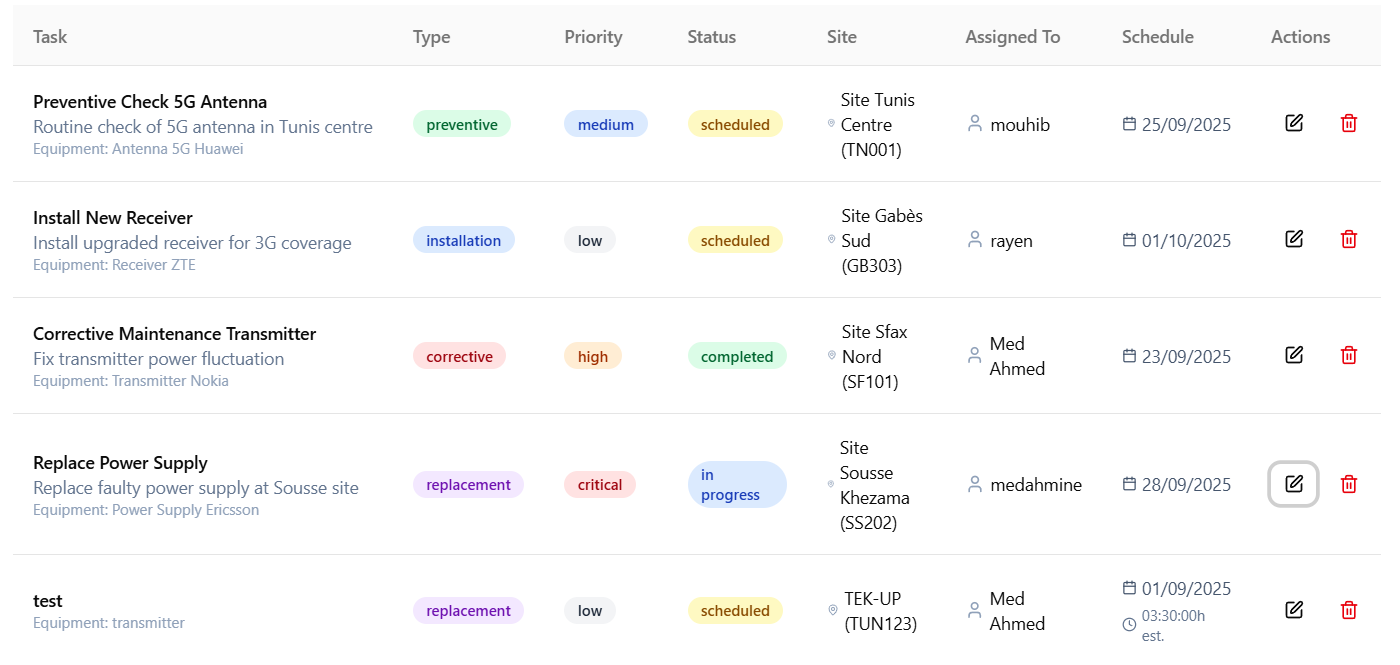
\includegraphics[width=0.7\textwidth]{img/chap_05/screenshot_schedule_intervention.png}}
\caption{Schedule intervention form with validation and conflict detection}
\label{fig:sprint3-impl3}
\end{figure}

The form includes fields for task title, intervention type, priority, target site, equipment selection, technician assignment, scheduled date, and estimated duration with comprehensive validation and conflict detection.

\subsection{Report Breakdown Form}

Figure \ref{fig:sprint3-impl4} shows the breakdown reporting form for incident documentation.

\begin{figure}[H]
\centering
\fbox{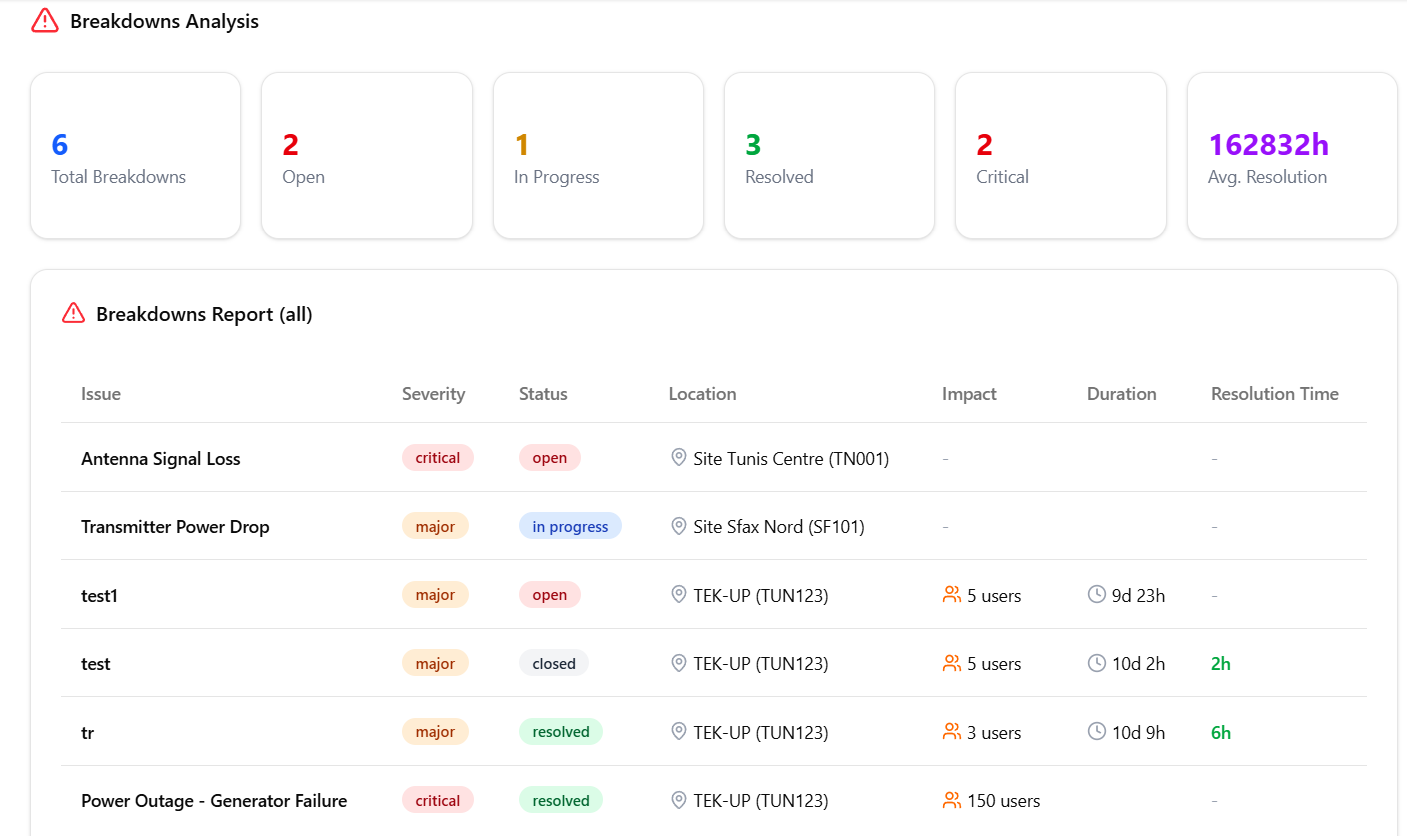
\includegraphics[width=0.7\textwidth]{img/chap_05/screenshot_report_breakdown.png}}
\caption{Report breakdown form with severity classification and impact estimation}
\label{fig:sprint3-impl4}
\end{figure}

The form enables quick incident reporting with breakdown type, severity classification, affected site and equipment selection, impact estimation, and automatic downtime tracking with critical severity escalation.

\section{Technical Challenges and Solutions}

\subsection{Technician Assignment Conflict Detection}

\textbf{Challenge:} Preventing double-booking when scheduling interventions required detecting time overlaps with variable-duration tasks stored as timestamps.

\textbf{Solution:} Implemented conflict detection algorithm querying existing interventions for assigned technician and checking time overlaps. The system calculates intervention end time by adding estimated duration to scheduled date, compares against proposed time slot, and displays warnings for conflicts while allowing managers flexibility in resource allocation.

\subsection{Real-time Downtime Duration Calculation}

\textbf{Challenge:} Displaying continuously updating breakdown duration in human-readable format without constant database queries or page refreshes.

\textbf{Solution:} Implemented client-side calculation function computing elapsed time from stored downtime start timestamp. The function intelligently formats durations: under 1 hour as "< 1h", under 24 hours as hours, and longer as days plus hours. The UI component recalculates periodically, providing accurate current information without database load.

\subsection{Cascading Status Updates and Timestamp Management}

\textbf{Challenge:} Multiple status transitions requiring automatic timestamp capture (acknowledged, resolved, closed) without manual entry while triggering related actions like downtime calculation.

\textbf{Solution:} Implemented automatic timestamp capture in update logic by detecting status changes and adding appropriate timestamp fields. When breakdown status becomes "investigating", system sets acknowledged timestamp; when "resolved", sets both resolved and downtime end timestamps enabling automatic duration calculation. This ensures data consistency and provides accurate audit trails.

\section{Testing and Validation}

\subsection{Functional Testing}

Functional testing verified all features work correctly. We tested breakdown reporting with various types and severities, confirming critical breakdowns trigger immediate manager notifications. Intervention scheduling validated different task types, technician assignment, and conflict detection. Status workflow transitions were tested through all states with automatic timestamp capture verification. CRUD operations for both breakdowns and interventions ensured data integrity.

\subsection{Integration Testing}

Integration testing ensured Sprint 3 components work with existing modules. We tested site and equipment integration by selecting resources when reporting breakdowns and scheduling interventions. Authentication and authorization were verified with different roles ensuring proper permission hierarchy. Real-time notifications confirmed managers receive critical breakdown alerts. Database relationships verified foreign key enforcement preventing orphaned records. Dashboard statistics validated accurate calculations.

\subsection{User Acceptance Testing}

Tunisia Telecom staff tested features in realistic scenarios. Technicians tested mobile-responsive interfaces for field reporting and confirmed easy form usage. Managers tested scheduling workflows, validating conflict detection and priority indicators. Engineers tested breakdown reporting with technical details, confirming adequate documentation fields and proper status transitions. Overall feedback was positive, with users appreciating clear visual indicators, intuitive workflows, and real-time updates.

\section{Conclusion}

Sprint 3 successfully delivered comprehensive breakdown management and intervention planning capabilities significantly enhancing TelecomOps maintenance functionality. The breakdown management system enables rapid incident reporting with detailed classification, automatic downtime tracking, and workflow-guided resolution. Critical severity escalation ensures urgent issues receive immediate attention, minimizing customer impact.

The intervention planning module enables preventive maintenance scheduling with technician assignment, progress tracking, and conflict detection preventing scheduling errors. Together, these modules create a complete maintenance solution balancing reactive and proactive approaches. Integration with existing modules ensures proper infrastructure association, while role-based permissions provide appropriate access levels. Real-time notifications keep stakeholders informed enabling rapid response.

Technical challenges around conflict detection and timestamp management were successfully resolved through careful validation logic and automatic data capture. Testing confirmed functional requirements and proper integration. Sprint 3 establishes foundation for advanced maintenance analytics and predictive capabilities, with comprehensive data enabling pattern analysis to optimize maintenance schedules and improve network reliability.